\documentclass[10pt,twocolumn]{article}
\usepackage[T1]{fontenc}
\usepackage[margin=0.72in]{geometry}
\usepackage{graphicx}
\usepackage{booktabs}
\usepackage{amsmath}
\usepackage{times}
\usepackage{caption}
\usepackage{url}
\usepackage[
  colorlinks=true,
  linkcolor=black,
  citecolor=black,
  urlcolor=blue,
  pdftitle={Not All Bad Demonstrations Are Equally Bad},
  pdfauthor={Jaiveer Bassi},
  pdfsubject={Demonstration quality in behaviour cloning},
  pdfkeywords={imitation learning, behaviour cloning, robot learning, data quality, policy evaluation}
]{hyperref}

\captionsetup{font=small,labelfont=bf}
\setlength{\parskip}{0pt}

\title{\vspace{-1.2em}\textbf{Not All Bad Demonstrations Are Equally Bad:}\\
Quantifying How Demonstration Failure Modes Degrade\\
Closed-Loop Policy Performance}

\author{Jaiveer Bassi\\
\small\url{https://github.com/imjbassi/demo-quality-robustness}}

\date{September 2026}

\begin{document}
\maketitle

\begin{abstract}
\noindent
Demonstration quality is often treated as a preprocessing concern in
imitation learning. We instead hold architecture, hyperparameters, episode
count, and evaluation conditions fixed while varying the type and prevalence
of defective demonstrations. Five failure modes---occlusion, accidental
success, corrective flailing, truncation, and inconsistent strategy---are
introduced into behaviour-cloning datasets for a controlled 2D block-pushing
task. Across 78 policy fits and three training seeds, outcomes differ sharply
by defect type. At full contamination, mean closed-loop success is $0.963$
for corrective flailing but $0.012$ for accidental success, compared with
$0.972$ for clean data. Accidental-success data retains mean success of
$0.890$ at $75\%$ contamination before collapsing at $100\%$. Pooled
open-loop action-prediction error correlates strongly with closed-loop success
($r=-0.91$), but within-mode correlations range from $-0.15$ to $-0.94$; in
the descriptive band $[0.20,0.30]$, similar open-loop errors
coincide with closed-loop success from $0.315$ to $0.980$. A control analysis
also rejects our initial interpretation of the inconsistent-strategy result:
the apparent degradation is explained by the alternate strategy's lower
clonability, not by mixing itself. These simulation results motivate
defect-specific quality control and closed-loop validation, while the small
seed count and simplified dynamics limit quantitative generalisation. Code,
raw results, and analysis are publicly available.
\end{abstract}

\section{Introduction}

Behaviour cloning is a standard baseline for robot manipulation
\cite{pomerleau1989alvinn}, and its central known weakness is compounding
error: small action errors move the policy off the demonstration distribution,
where its predictions degrade further \cite{ross2011dagger}. The standard
responses to this are architectural or algorithmic: better policy classes
\cite{chi2023diffusion}, or interactive data collection.

Practitioners running data-collection pipelines know something the literature
under-quantifies: the demonstrations themselves fail in structured,
recognisable ways. A camera is occluded mid-episode. An operator fumbles and
the object lands on the goal anyway. Two operators solve the same task with
incompatible strategies. An episode is cut short. These are not Gaussian noise
on a clean signal; they are distinct defects with distinct structure, and
quality-control effort spent on one is effort not spent on another.

Prior work has established that demonstration quality matters in aggregate
\cite{mandlekar2021what,belkhale2023data}. What is less established is a
\emph{ranking}: given finite QC budget, which defect should a pipeline
prioritise? And, because closed-loop evaluation is expensive and open-loop
action-prediction error is cheap, does the cheap metric even detect the
damage?

This paper answers both questions in a deliberately small, fully controlled
setting. Our contributions are:

\begin{enumerate}\itemsep2pt
\item A controlled experimental design treating demonstration quality as the
independent variable, with contamination rate as a single comparable axis
across five distinct failure modes.
\item A descriptive ranking of failure modes by closed-loop degradation in a
controlled block-pushing setting.
\item Evidence that a strong pooled association between open- and closed-loop
metrics does not imply uniform diagnostic value within each failure mode.
\item A control analysis showing that an apparent strategy-inconsistency
effect is instead explained by unequal strategy clonability.
\end{enumerate}

\section{Method}

\subsection{Environment}

\textbf{Push2D} is a 2D block-pushing task implemented in vectorised NumPy. A
point gripper must move a block into a goal region. Pushing was chosen over
reaching deliberately: it imposes a \emph{staging} requirement, since the
gripper must position itself behind the block relative to the goal before
pushing is productive. This makes compounding error consequential. A policy
that drifts during approach ends up on the wrong side and pushes the block
\emph{away} from the goal, which is unrecoverable within the episode budget.
This is precisely the class of failure that open-loop metrics are structurally
poor at surfacing, since each individual action error is small.

Observations are 10-dimensional (gripper, block and goal positions plus two
relative vectors); actions are 2D displacements clipped to $[-1,1]$. Episodes
run for at most 110 steps and terminate on success, defined as the block
centre falling within $0.05$ of the goal.

\subsection{Scripted experts}

Using scripted rather than human demonstrations is what makes the experiment
controlled: corruption can be applied with exact, programmatic ground truth
rather than human judgement about what counts as a bad demo.

The \textbf{primary expert} is a hand-coded orbit-then-push controller that
circles the block at a safe radius until aligned, then pushes toward the goal.
Measured success rate: $\mathbf{100.0\%}$.

The \textbf{alternate expert} always circles in the same rotational direction
from a wider staging radius, producing a visibly different route through state
space. It was explicitly tuned until it \emph{also} reaches
$\mathbf{100.0\%}$, so that mixing the two tests strategy \emph{inconsistency}
rather than strategy \emph{quality}. This tuning turns out to matter
substantially (Section~\ref{sec:failed}).

The \textbf{naive controller} charges blindly at the block and never reasons
about the goal; the block travels along whatever ray the gripper started on.
It succeeds on approximately 6\% of episodes, purely by geometric luck.

\subsection{Failure modes}

Each mode produces demonstrations that a real pipeline could plausibly log:

\textbf{Occlusion.} A contiguous window covering 35\% of timesteps has its
observations frozen at the last visible frame. Actions remain
expert-quality; the demonstrator can see, the camera cannot. The resulting
transitions have corrupted inputs and pristine labels.

\textbf{Accidental success.} Rollouts from the naive controller, keeping only
those that reached the goal. Correct outcome, no correct behaviour anywhere in
the episode.

\textbf{Corrective flailing.} Heavy uniform jitter on the first 12 timesteps,
after which the demonstrator settles into correct motion and still succeeds.

\textbf{Truncation.} A clean episode cut at 70\% of its length and logged
anyway, what a QC filter missing a premature stop looks like.

\textbf{Inconsistent strategy.} Complete episodes from the alternate expert.
Every one is a genuine success; the only defect is disagreement with the
primary strategy about what to do in a given state.

\subsection{Two design decisions}

\textbf{Action-level corruptions are re-simulated, not pasted.} Overwriting
actions in a logged trajectory without re-running the dynamics yields
observations that no longer follow from the actions, a physically impossible
episode. That measures label noise, not bad demonstrations. Every mode that
touches actions replays the episode through the environment.

\textbf{Corrupted episodes must pass the same success-based QC filter a real
pipeline applies.} Modes are rejection-sampled to successful episodes only.
Truncation is the deliberate exception, since it \emph{is} the filter failing.

\subsection{Sweep axis, policy and evaluation}

The sweep axis is \textbf{contamination rate} $\rho$, not per-episode
severity. Every dataset contains the same number of episodes; $\rho$ of them
are defective and $(1-\rho)$ are clean, with per-episode severity held fixed.
This places all five modes on one comparable axis and answers the question a
pipeline actually asks: what fraction of the dataset can be this kind of bad
before the policy breaks?

We sweep $\rho \in \{0, 0.25, 0.5, 0.75, 0.9, 1.0\}$ across three training
seeds. The shared clean baseline is fitted once per seed, giving 78 distinct
policy fits: three clean fits and $5\times5\times3$ contaminated fits. Every
run uses an identical $2\times256$ ReLU MLP trained
with MSE behaviour cloning for 50 epochs on 400 episodes ($\approx$13k
transitions). The model is deliberately small: it is not the independent
variable.

Two metrics are recorded per policy. \textbf{Open-loop MSE} is
action-prediction error against the expert on held-out \emph{clean} expert
states (cheap, offline, no environment interaction). \textbf{Closed-loop
success rate} runs the policy in the environment over 200 episodes. The same
200 evaluation initial conditions are reused for every configuration to
support paired descriptive comparisons.

\begin{figure*}[t]
\centering
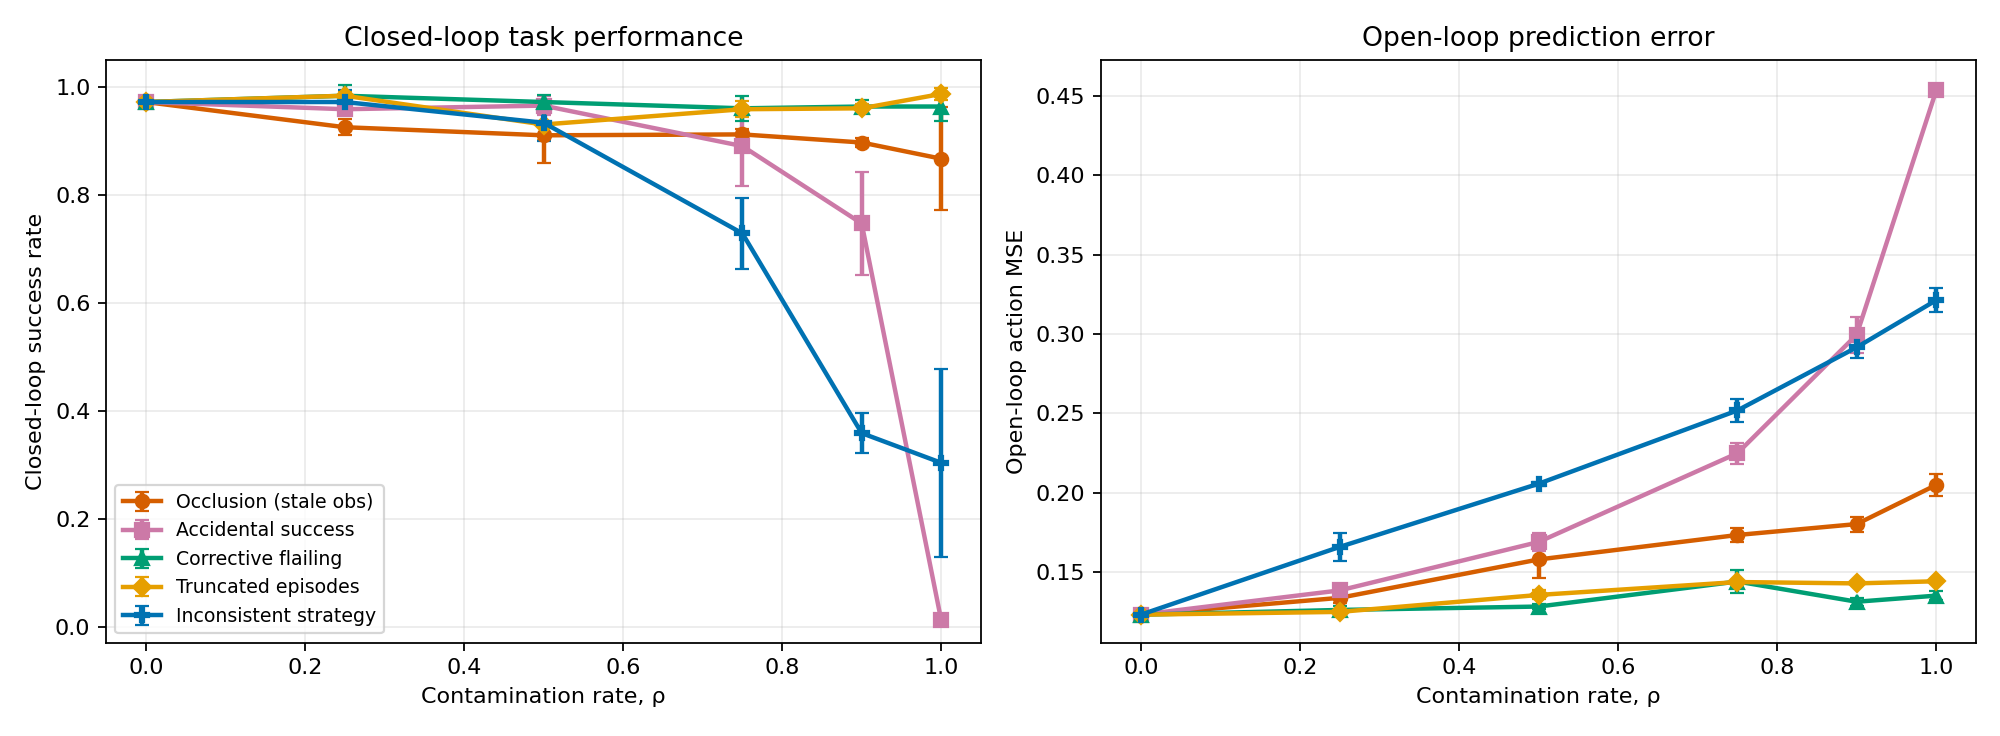
\includegraphics[width=\textwidth]{results/fig1_dose_response.png}
\caption{Dose--response curves across contamination rate. \textbf{Left:}
closed-loop success rate, the quantity of interest. \textbf{Right:} open-loop
MSE, the offline proxy. Accidental-success policies retain high mean success at
$\rho=0.75$ before collapsing at $\rho=1.0$, whereas corrective flailing and
truncation remain comparatively stable. Points are means and error bars are
standard deviations over three training seeds.}
\label{fig:dose}
\end{figure*}

\section{Results}

The clean baseline reaches $0.972 \pm 0.010$ closed-loop success (mean $\pm$
standard deviation over three training seeds). All uncertainty summaries are
descriptive; the small seed count does not support formal significance claims.

\subsection{Failure modes are not interchangeable}

Table~\ref{tab:main} gives the headline comparison. At full contamination,
corrective flailing reduces mean success by $0.009$ relative to the clean
baseline, whereas accidental success reduces it by $0.960$. Both are ``bad
demonstrations'' under a practical taxonomy, yet their observed costs differ
by two orders of magnitude.

\textbf{Corrective flailing causes little degradation in this setting.}
Jitter-then-recover trajectories may provide DAgger-like coverage of
off-distribution states \cite{ross2011dagger}; at $\rho=1.0$, mean success is
$0.963$, close to the clean baseline. This pattern makes corrective flailing a
lower QC priority here, although three seeds are insufficient to establish
equivalence or benefit.

\textbf{Truncation does not reduce mean success in the observed setting}:
mean success is $0.987$ at $\rho=1.0$. A plausible explanation is that the push action can be
extrapolated from the retained approach phase. This interpretation should not
be transferred to tasks with a distinct terminal phase, such as grasping,
without further experiments.

\begin{table}[t]
\centering
\small
\begin{tabular}{@{}lccc@{}}
\toprule
\textbf{Failure mode} & $\rho{=}0.5$ & $\rho{=}1.0$ & Pearson $r$ \\
\midrule
Corrective flailing    & 0.972 & 0.963 & $-0.35$ \\
Truncated episodes     & 0.930 & 0.987 & $-0.15$ \\
Occlusion (stale obs)  & 0.910 & 0.867 & $-0.58$ \\
Inconsistent strategy  & 0.933 & 0.303 & $-0.90$ \\
Accidental success     & 0.965 & \textbf{0.012} & $-0.94$ \\
\midrule
\textit{Clean baseline} & \multicolumn{2}{c}{\textit{0.972}} & n/a \\
\bottomrule
\end{tabular}
\caption{Closed-loop success rate by failure mode and contamination rate, mean
over three seeds. Pearson $r$ is the within-mode correlation between open-loop
MSE and closed-loop success across all runs of that mode.}
\label{tab:main}
\end{table}

\subsection{Accidental success is a cliff, not a slope}

The most operationally significant observed result is the shape of the accidental
success curve: $0.965$ at $\rho=0.5$, $0.890$ at $\rho=0.75$, $0.747$ at
$\rho=0.9$, and $\mathbf{0.012}$ at $\rho=1.0$.

In this experiment, a minority of clean demonstrations masks much of the
problem. A pipeline monitoring only success-labelled demonstration throughput
would not reveal the approaching policy failure. The
diagnostic wrong-side push rate tells the same story, rising from $0.008$ at
$\rho=0.5$ to $0.468$ at $\rho=1.0$: the policy has learned to shove the block
in essentially arbitrary directions.

\subsection{Open-loop evaluation has failure-mode-dependent value}

Pooled across all 78 distinct policy fits, open-loop MSE correlates with
closed-loop success at $r=-0.91$. This strong aggregate association could
appear to justify its use as a screening metric.

Broken out by failure mode, however, Pearson correlations range from $-0.15$
(truncation) to $-0.94$ (accidental success). The metric is strongly
associated with success for some defects but weakly associated for truncation
and corrective flailing, precisely where closed-loop performance varies
little.

A complementary descriptive comparison considers the 15 runs whose open-loop
MSE falls in the descriptive band $[0.20,0.30]$. Their closed-loop success
ranges from $\mathbf{0.315}$ to $\mathbf{0.980}$. This band is not a
statistical equivalence test; it illustrates that numerically similar offline
scores need not determine similar task outcomes. Figure~\ref{fig:scatter}
shows the full distribution, including the high-MSE collapse points that
contribute strongly to the pooled correlation.

\begin{figure}[t]
\centering
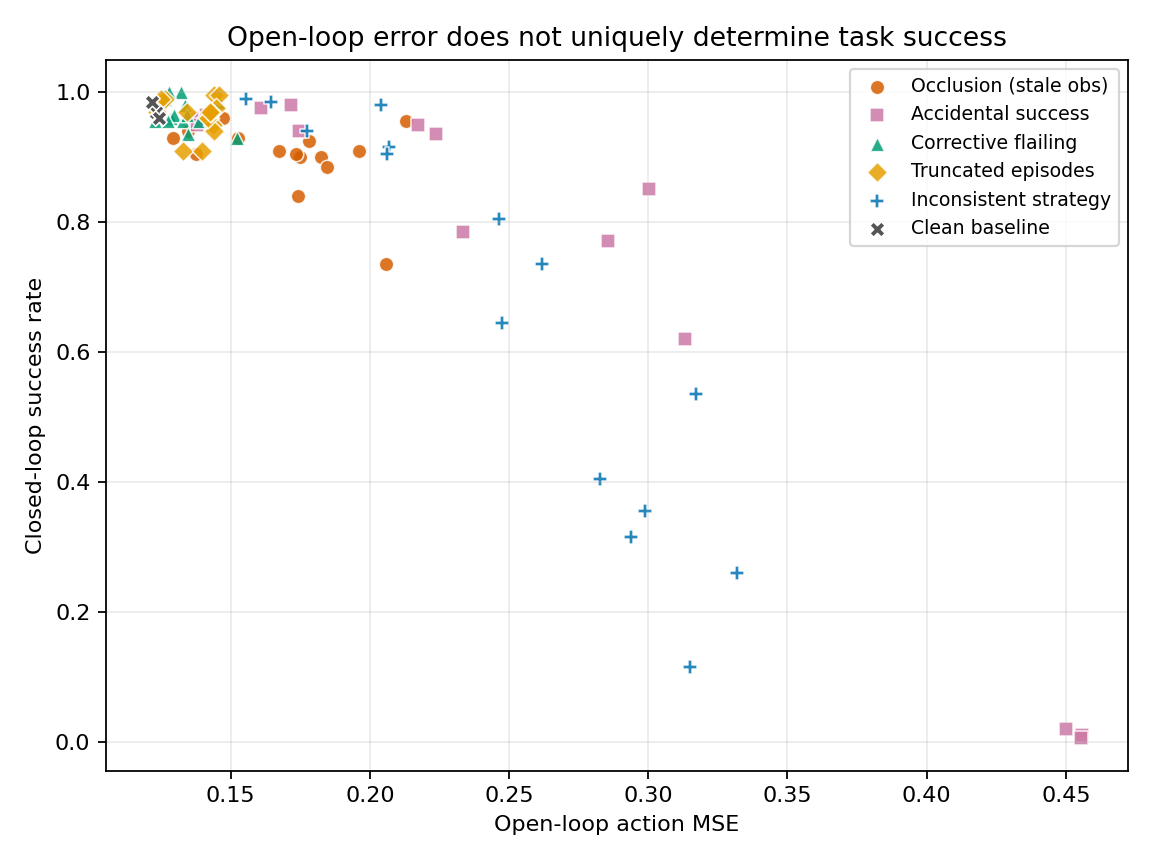
\includegraphics[width=\columnwidth]{results/fig2_openloop_vs_closedloop.png}
\caption{Open-loop MSE against closed-loop success for all 78 distinct policy
fits. Within the descriptive MSE band $[0.20,0.30]$, closed-loop success spans
$0.665$.}
\label{fig:scatter}
\end{figure}

\section{A prediction that failed}
\label{sec:failed}

We predicted that mixing two valid strategies would cause multimodal-averaging
collapse, since an MSE-regression policy averages conflicting action targets by
construction. The data does not support this, and the control is worth stating
explicitly because it nearly produced a false positive.

At $\rho=1.0$ the dataset is entirely alternate-strategy and therefore fully
self-consistent; there is no mixing left to blame. Success there ($0.303$) is
the \emph{clonability floor} of that strategy, not evidence of inconsistency
harm. Both experts solve the task on 100\% of episodes; the alternate is
simply harder to clone, having a longer horizon and more orbit steps over
which error compounds.

Reading intermediate $\rho$ against the line joining the two endpoints
isolates any harm attributable to mixing:

\begin{table}[h]
\centering
\small
\begin{tabular}{@{}cccc@{}}
\toprule
$\rho$ & Observed & Interpolated & Residual \\
\midrule
0.25 & 0.972 & 0.805 & $+0.167$ \\
0.50 & 0.933 & 0.637 & $+0.296$ \\
0.75 & 0.728 & 0.470 & $+0.258$ \\
0.90 & 0.358 & 0.370 & $-0.012$ \\
\bottomrule
\end{tabular}
\caption{Observed success relative to linear interpolation between the
$\rho=0$ and $\rho=1$ endpoints. Positive residuals indicate performance
\emph{above}, not below, the clonability-only interpolation.}
\label{tab:clon}
\end{table}

The residual is non-negative at three of four intermediate points and slightly
negative at $\rho=0.9$. Thus, the observations provide no consistent evidence
that mixing is worse than the clonability-only interpolation; at lower
contamination rates, clean data may instead be protective. The
inconsistent-strategy curve in
Figure~\ref{fig:dose} looks damaging only because one of the two strategies is
intrinsically harder to imitate.

This control materially qualifies the headline comparison. Removing the
inconsistent-strategy runs from the matched-MSE band narrows the closed-loop
spread from $0.665$ to approximately $0.22$. This narrower descriptive spread
is considerably more modest than the raw figure suggests.

\section{Limitations}

\textbf{Three training seeds are insufficient for precise inference.} Some
cells are noisy: occlusion at $\rho=1.0$ spans $0.735$ to $0.955$ across
seeds. The means and standard deviations therefore describe these runs rather
than establish population-level effects; confirmatory work should use more
seeds and report uncertainty intervals.

\textbf{One fixed evaluation set.} Reusing the same 200 initial conditions
reduces between-configuration nuisance variation but does not measure
sensitivity to the evaluation-state distribution. Replication should vary
both training and evaluation seeds.

\textbf{A 2D toy environment.} Whether these rankings survive in a 7-DOF
setting with contact dynamics and visual observations is open. This work
establishes a methodology, not transferable constants.

\textbf{One policy class.} MSE regression averages multimodal action
distributions by construction. The inconsistent-strategy result in particular
may be specific to this choice; replicating it with a diffusion policy
\cite{chi2023diffusion} is the most informative single follow-up.

\textbf{Transition imbalance.} Alternate-strategy episodes are longer, so at
fixed episode count they contribute more transitions. A transition-matched
replication would tighten that arm further.

\section{Conclusion}

Treating demonstration quality as the independent variable, rather than an
implementation detail, produces a defect-specific ranking in this controlled
task: accidental-success performance collapses near full contamination,
occlusion produces a moderate decline, and corrective flailing and truncation
remain comparatively stable. The practical hypothesis for larger systems is
that QC effort should be allocated by defect type rather than uniformly.

The evaluation result is equally important: open-loop action-prediction error
has a strong pooled association with closed-loop success, yet its diagnostic
value varies substantially by failure mode. Offline screening is useful, but
it is not a substitute for closed-loop validation.

\section*{Reproducibility statement}

Source code, exact training and evaluation seeds, raw per-run results, and the
scripts used to generate both figures are available at
\url{https://github.com/imjbassi/demo-quality-robustness}. The repository also
records the software requirements and commands needed to reproduce all 78
policy fits and rebuild this manuscript.

\begin{thebibliography}{9}
\small
\bibitem{pomerleau1989alvinn}
D.~Pomerleau. ALVINN: An Autonomous Land Vehicle in a Neural Network.
\textit{NeurIPS}, 1989.

\bibitem{ross2011dagger}
S.~Ross, G.~Gordon, and D.~Bagnell. A Reduction of Imitation Learning and
Structured Prediction to No-Regret Online Learning. \textit{AISTATS}, 2011.

\bibitem{mandlekar2021what}
A.~Mandlekar et al. What Matters in Learning from Offline Human
Demonstrations for Robot Manipulation. \textit{CoRL}, 2021.

\bibitem{belkhale2023data}
S.~Belkhale, Y.~Cui, and D.~Sadigh. Data Quality in Imitation Learning.
\textit{NeurIPS}, 2023.

\bibitem{chi2023diffusion}
C.~Chi et al. Diffusion Policy: Visuomotor Policy Learning via Action
Diffusion. \textit{RSS}, 2023.
\end{thebibliography}

\end{document}
